\documentclass[11pt,a4paper]{article}
%%%%%%%%%%%%%%%%%%%%%%%%%%%%%%%%%%%%%%%%%%%%%%%%%%%%%%%%
%                      PACKAGES                        %
%%%%%%%%%%%%%%%%%%%%%%%%%%%%%%%%%%%%%%%%%%%%%%%%%%%%%%%%

\usepackage[utf8]{inputenc}
\usepackage{graphicx} % Allows you to insert figures
\usepackage[export]{adjustbox}
\usepackage{booktabs}
\usepackage{amsmath} % Allows you to do equations
\usepackage{helvet}
\usepackage{hyperref}
\renewcommand{\familydefault}{\sfdefault}
\usepackage[a4paper, total={6.5in, 9.5in}]{geometry} % Formats the paper size, orientation, and margins
\linespread{1.1} % about 1.5 spacing in Word
\setlength{\parindent}{0pt} % no paragraph indents
\setlength{\parskip}{1em} % paragraphs separated by one line
\usepackage{listings}
\usepackage{enumitem}
\usepackage{xcolor}
\usepackage{hyperref}
\hypersetup{
	colorlinks=true,
	urlcolor=cyan,
	linktoc=none,
}
\usepackage{fancyhdr}
\pagestyle{fancy}
\fancyhead[L,C,R]{}
\fancyfoot[L]{Blix - AI Photo Editor}
\fancyfoot[C]{}
\fancyfoot[R]{\textbf{\thepage}}
\renewcommand{\headrulewidth}{0pt}
\renewcommand{\footrulewidth}{0.5pt}

\definecolor{codegreen}{rgb}{0,0.6,0}
\definecolor{codegray}{rgb}{0.5,0.5,0.5}
\definecolor{codepurple}{rgb}{0.58,0,0.82}
\definecolor{backcolour}{rgb}{0.95,0.95,0.92}

\lstdefinestyle{mystyle}{
backgroundcolor=\color{backcolour},
commentstyle=\color{codegreen},
keywordstyle=\color{magenta},
numberstyle=\tiny\color{codegray},
stringstyle=\color{codepurple},
basicstyle=\ttfamily\footnotesize,
breakatwhitespace=false,
breaklines=true,
keepspaces=true,
numbers=left,
numbersep=5pt,
showspaces=false,
showstringspaces=false,
showtabs=false,
tabsize=2,
}

\lstset{style=mystyle}
\def\code#1{\texttt{#1}}

%%%%%%%%%%%%%%%%%%%%%%%%%%%%%%%%%%%%%%%%%%%%%%%%%%%%%%%%
%            TITLE PAGE & TABLE OF CONTENTS            %
%%%%%%%%%%%%%%%%%%%%%%%%%%%%%%%%%%%%%%%%%%%%%%%%%%%%%%%%

\begin{document}

\begin{titlepage}
	\centering
    % \includegraphics[width=0.5\textwidth]{your_logo.png}\par\vspace{1cm}
    {\scshape\LARGE Software Requirements Specification\par}
    \vspace{1.5cm}
    {\huge\bfseries Blix - AI Photo Editor\par}
    \begin{figure}[h]
        \centering % center the image
        
\includegraphics[width=0.5\textwidth]{../pics/blix.png}
    \end{figure}
    \vspace{2.5cm}
    {\Large\itshape The Spanish Inquisition\par}
	\begin{tabular}{|c|c|}
		\hline
		\textbf{Name} 		& \textbf{Student Number} \\
		\hline
		Armand Krynauw		& u04868286  \\
		Jake Mileham		& u21692492  \\
		Dino Gironi			& u21630276  \\
		Karel Olwage		& u21555258  \\
		Francois Combrinck	& u21729752  \\
		\hline
	\end{tabular}
    \vfill
    {\large \today\par}
\end{titlepage}

\tableofcontents
\pagebreak

%%%%%%%%%%%%%%%%%%%%%%%%%%%%%%%%%%%%%%%%%%%%%%%%%%%%%%%%
%                MAIN DOCUMENT CONTENT                 %
%%%%%%%%%%%%%%%%%%%%%%%%%%%%%%%%%%%%%%%%%%%%%%%%%%%%%%%%

\addcontentsline{toc}{section}{Introduction}
\section*{Introduction}

Blix is a native cross-platform desktop application designed to provide users
with a powerful and intuitive photo editing experience.

\addcontentsline{toc}{subsection}{Purpose and Vision}
\subsection*{Purpose and Vision}

In photography, editing is an essential part of the process. However, it can be
time-consuming and daunting, especially for those unfamiliar with the techniques
and software. 

Blix is a native, cross-platform desktop application designed to give users a
powerful, intuitive photo editing experience. It enables users to edit photos 
using a node-based system, which describes the image processing pipeline. This
offers creative control to professionals, while still being intuitive for 
novice users.

Domain Pulse is the ultimate sentiment analysis platform. It gathers and analyses
online opinions about any domain, be it a business, a person, or more. With stunning
visuals and easy-to-understand statistics, Domain Pulse helps you understand the
online presence and sentiment for any domain

The system provides functionality for basic photo editing operations, like white
balance and saturation. It also has advanced operations, such as image
segmentation, which allows users to edit selected objects individually and
provides infilling. 

Users can customize the themes and layout of the application. The viewport is
splittable and users can arrange components throughout the window layout. It has
a command palette which enables users to efficiently navigate and control the
system. This allows users to change themes, add nodes to the graph, manage
projects and more. It also has a custom AI prompt box where users can describe
their vision of the image, which will then be processed to generate a result.

The system also allows users to sync their photo editing projects and user
preferences to the cloud, including window layout, keymap settings and themes.

\pagebreak


\addcontentsline{toc}{section}{User Stories and Characteristics}
\section*{User Stories and Characteristics}

\addcontentsline{toc}{subsection}{Characteristics}
\subsection*{Characteristics}

\subsubsection*{Novice Users}

Novice users are typically individuals who have little to no experience with
photo editing software. They may be unfamiliar with the terminology and tools
used in the application, and may require guidance and assistance with basic
tasks such as importing and exporting photos, adjusting brightness and contrast,
cropping and resizing images, and applying filters and effects. Novice users may
also be less comfortable with technology in general, and may require a more
intuitive and user-friendly interface to help them navigate the application.


\subsubsection*{Intermediate Users}

An intermediate user is someone who has a good understanding of the basic
features and tools of the application, but may not be familiar with more
advanced techniques. They are likely to have experience with editing photos and
may have used similar applications before. They are comfortable navigating the
interface and using tools such as crop, resize, and color adjustments. They may
also be interested in learning more advanced techniques such as layering,
masking, and retouching to enhance their photos. 

\subsubsection*{Professional Users}

A professional user of a photo editing application is typically someone who has
a deep understanding of photography and image editing techniques. They are
likely to have experience using a variety of photo editing software and are
proficient in using advanced features such as layers, masks, and color
correction tools. They may work in fields such as graphic design, advertising,
or photography and require a high level of precision and control over their
edits. Professional users may also value features such as batch processing and
the ability to work with large files or RAW image formats. They may also
prioritize software that integrates well with other tools in their workflow,
such as design software or cloud storage services.

\pagebreak

\addcontentsline{toc}{subsection}{Stories}
\subsection*{Stories}

\subsubsection*{Novice users}

I want the application to have a simple and intuitive interface, so that I can
easily navigate and understand how to use it.

I want the application to provide basic editing tools, such as crop and rotate,
so that I can quickly make simple adjustments to my photos.

I want the application to offer a variety of pre-set filters and effects, so
that I can easily enhance the look of my photos without needing to learn
advanced editing techniques.

\subsubsection*{Intermediate users}

I want the application to offer more advanced editing tools, such as levels and
curves, so that I can fine-tune the exposure and color of my photos.

I want the application to provide a range of creative options, such as overlays
and textures, so that I can experiment with different styles and effects.

I want the application to provide easy sharing options, so that I can quickly
post my edited photos to my favorite platforms.

I want to be able to upload and edit multiple photos at once.

I want to be able to adjust advanced settings such as white balance, hue,
exposure, cropping, and rotating manually.

I want to be able to select objects in the image using image segmentation and
edit them separately.

I want to be able to search for projects by the content of the images inside of
them.

I want to be able to customize the panel layout to my preference.


\subsubsection*{Professional users}

I want the application to offer advanced retouching tools, such as frequency
separation and dodge and burn, so that I can make precise adjustments to my
photos.

I want the application to support high-resolution files and offer advanced color
management options, so that I can create professional-quality designs.

I want the application to provide batch processing and automation options, so
that I can quickly edit and optimize large numbers of photos for use in
campaigns and advertisements.

\pagebreak

\addcontentsline{toc}{section}{Class Diagrams}
\section*{Class Diagrams}

\addcontentsline{toc}{subsection}{Project Management Subsystem}
\subsubsection*{Project Management Subsystem}
\begin{figure}[htbp]
    \centering
    \href{https://drive.google.com/drive/u/2/folders/1rnYMSGTOmKY8_pOyJUIacjTxuubO_6NX}
    {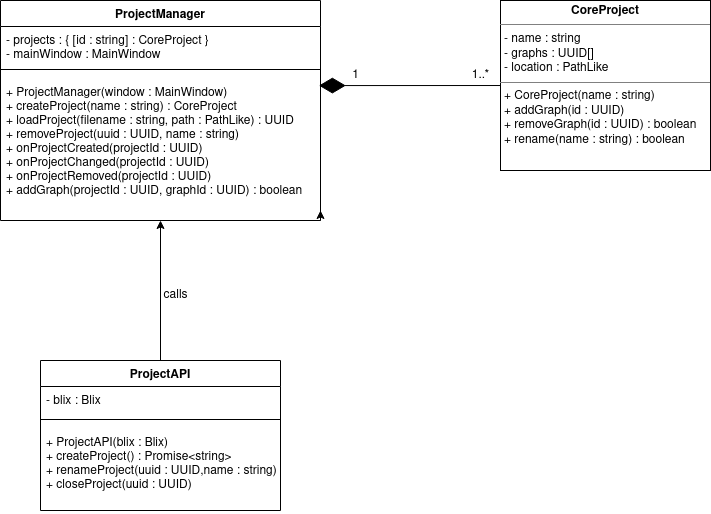
\includegraphics[width=0.55\textwidth]{../diagramPng/Project-subsystem.png}}
\end{figure}

\addcontentsline{toc}{subsection}{Layout Subsystem}
\subsubsection*{Layout Subsystem}
\begin{figure}[htbp]
    \centering
      \href{https://drive.google.com/drive/u/2/folders/1rnYMSGTOmKY8_pOyJUIacjTxuubO_6NX}
      {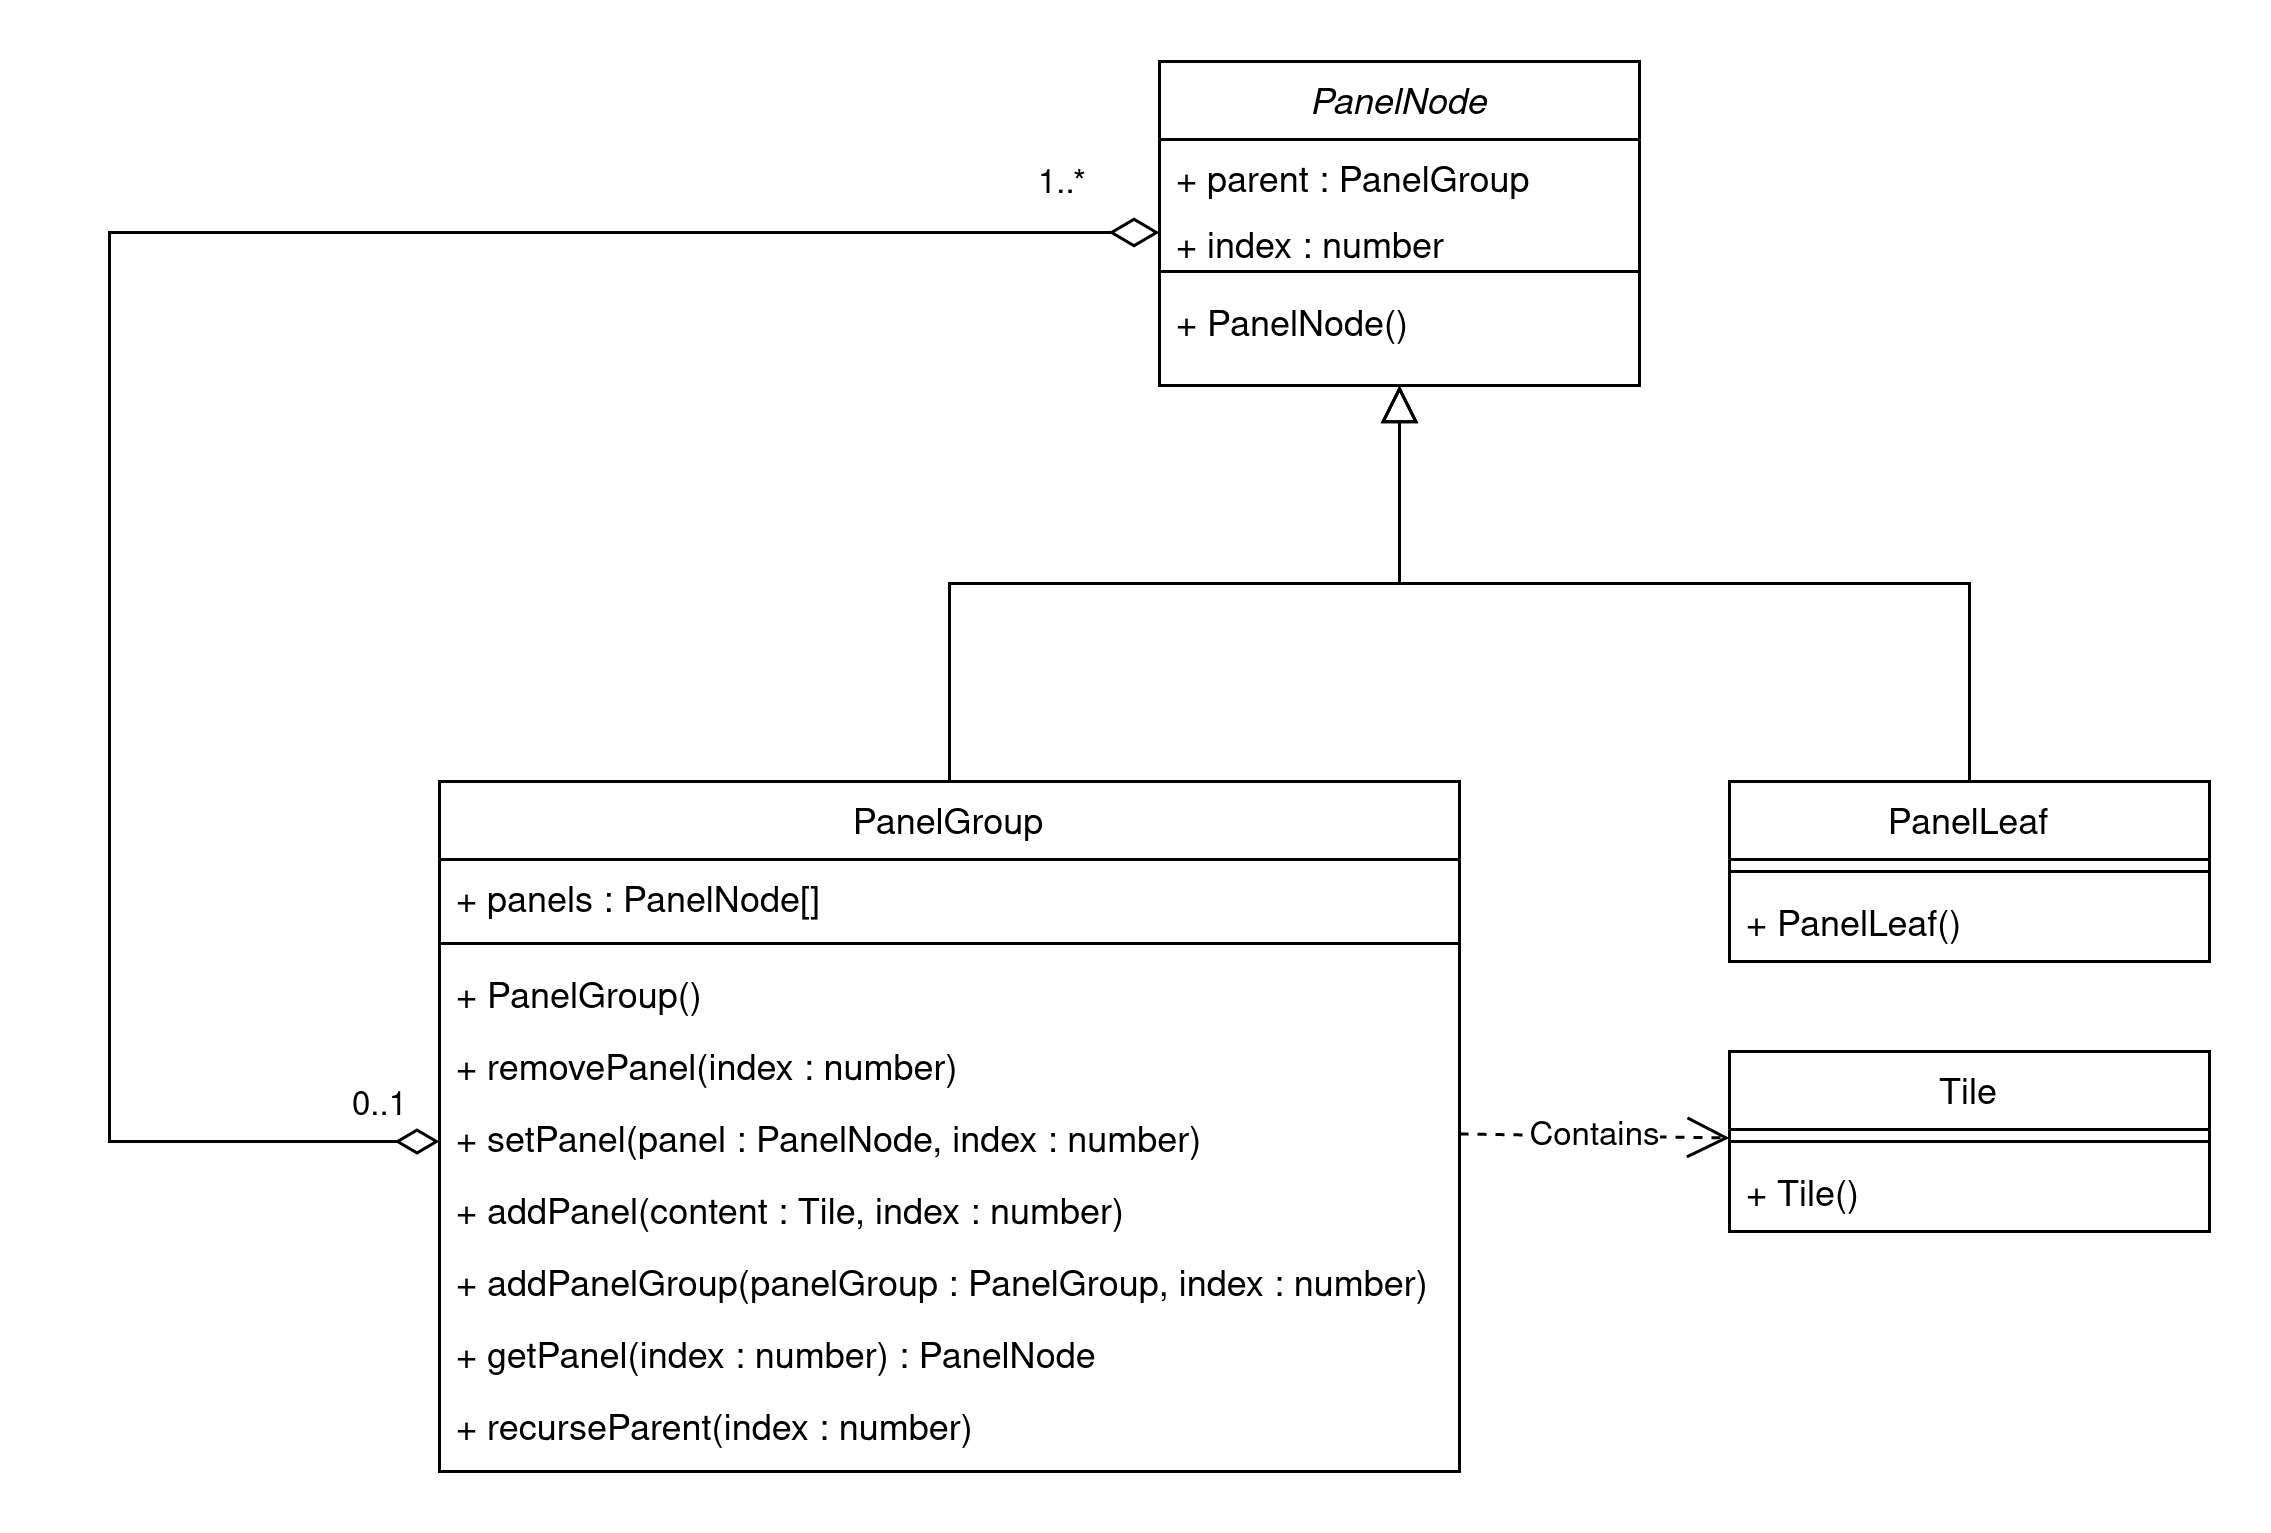
\includegraphics[width=0.8\textwidth]{../diagramPng/Layout-Subsystem.png}}
\end{figure}

\addcontentsline{toc}{subsection}{Graph Management Subsystem}
\subsubsection*{Graph Management Subsystem}
\begin{figure}[htbp]
  \centering
  \href{https://drive.google.com/drive/u/2/folders/1rnYMSGTOmKY8_pOyJUIacjTxuubO_6NX}
  {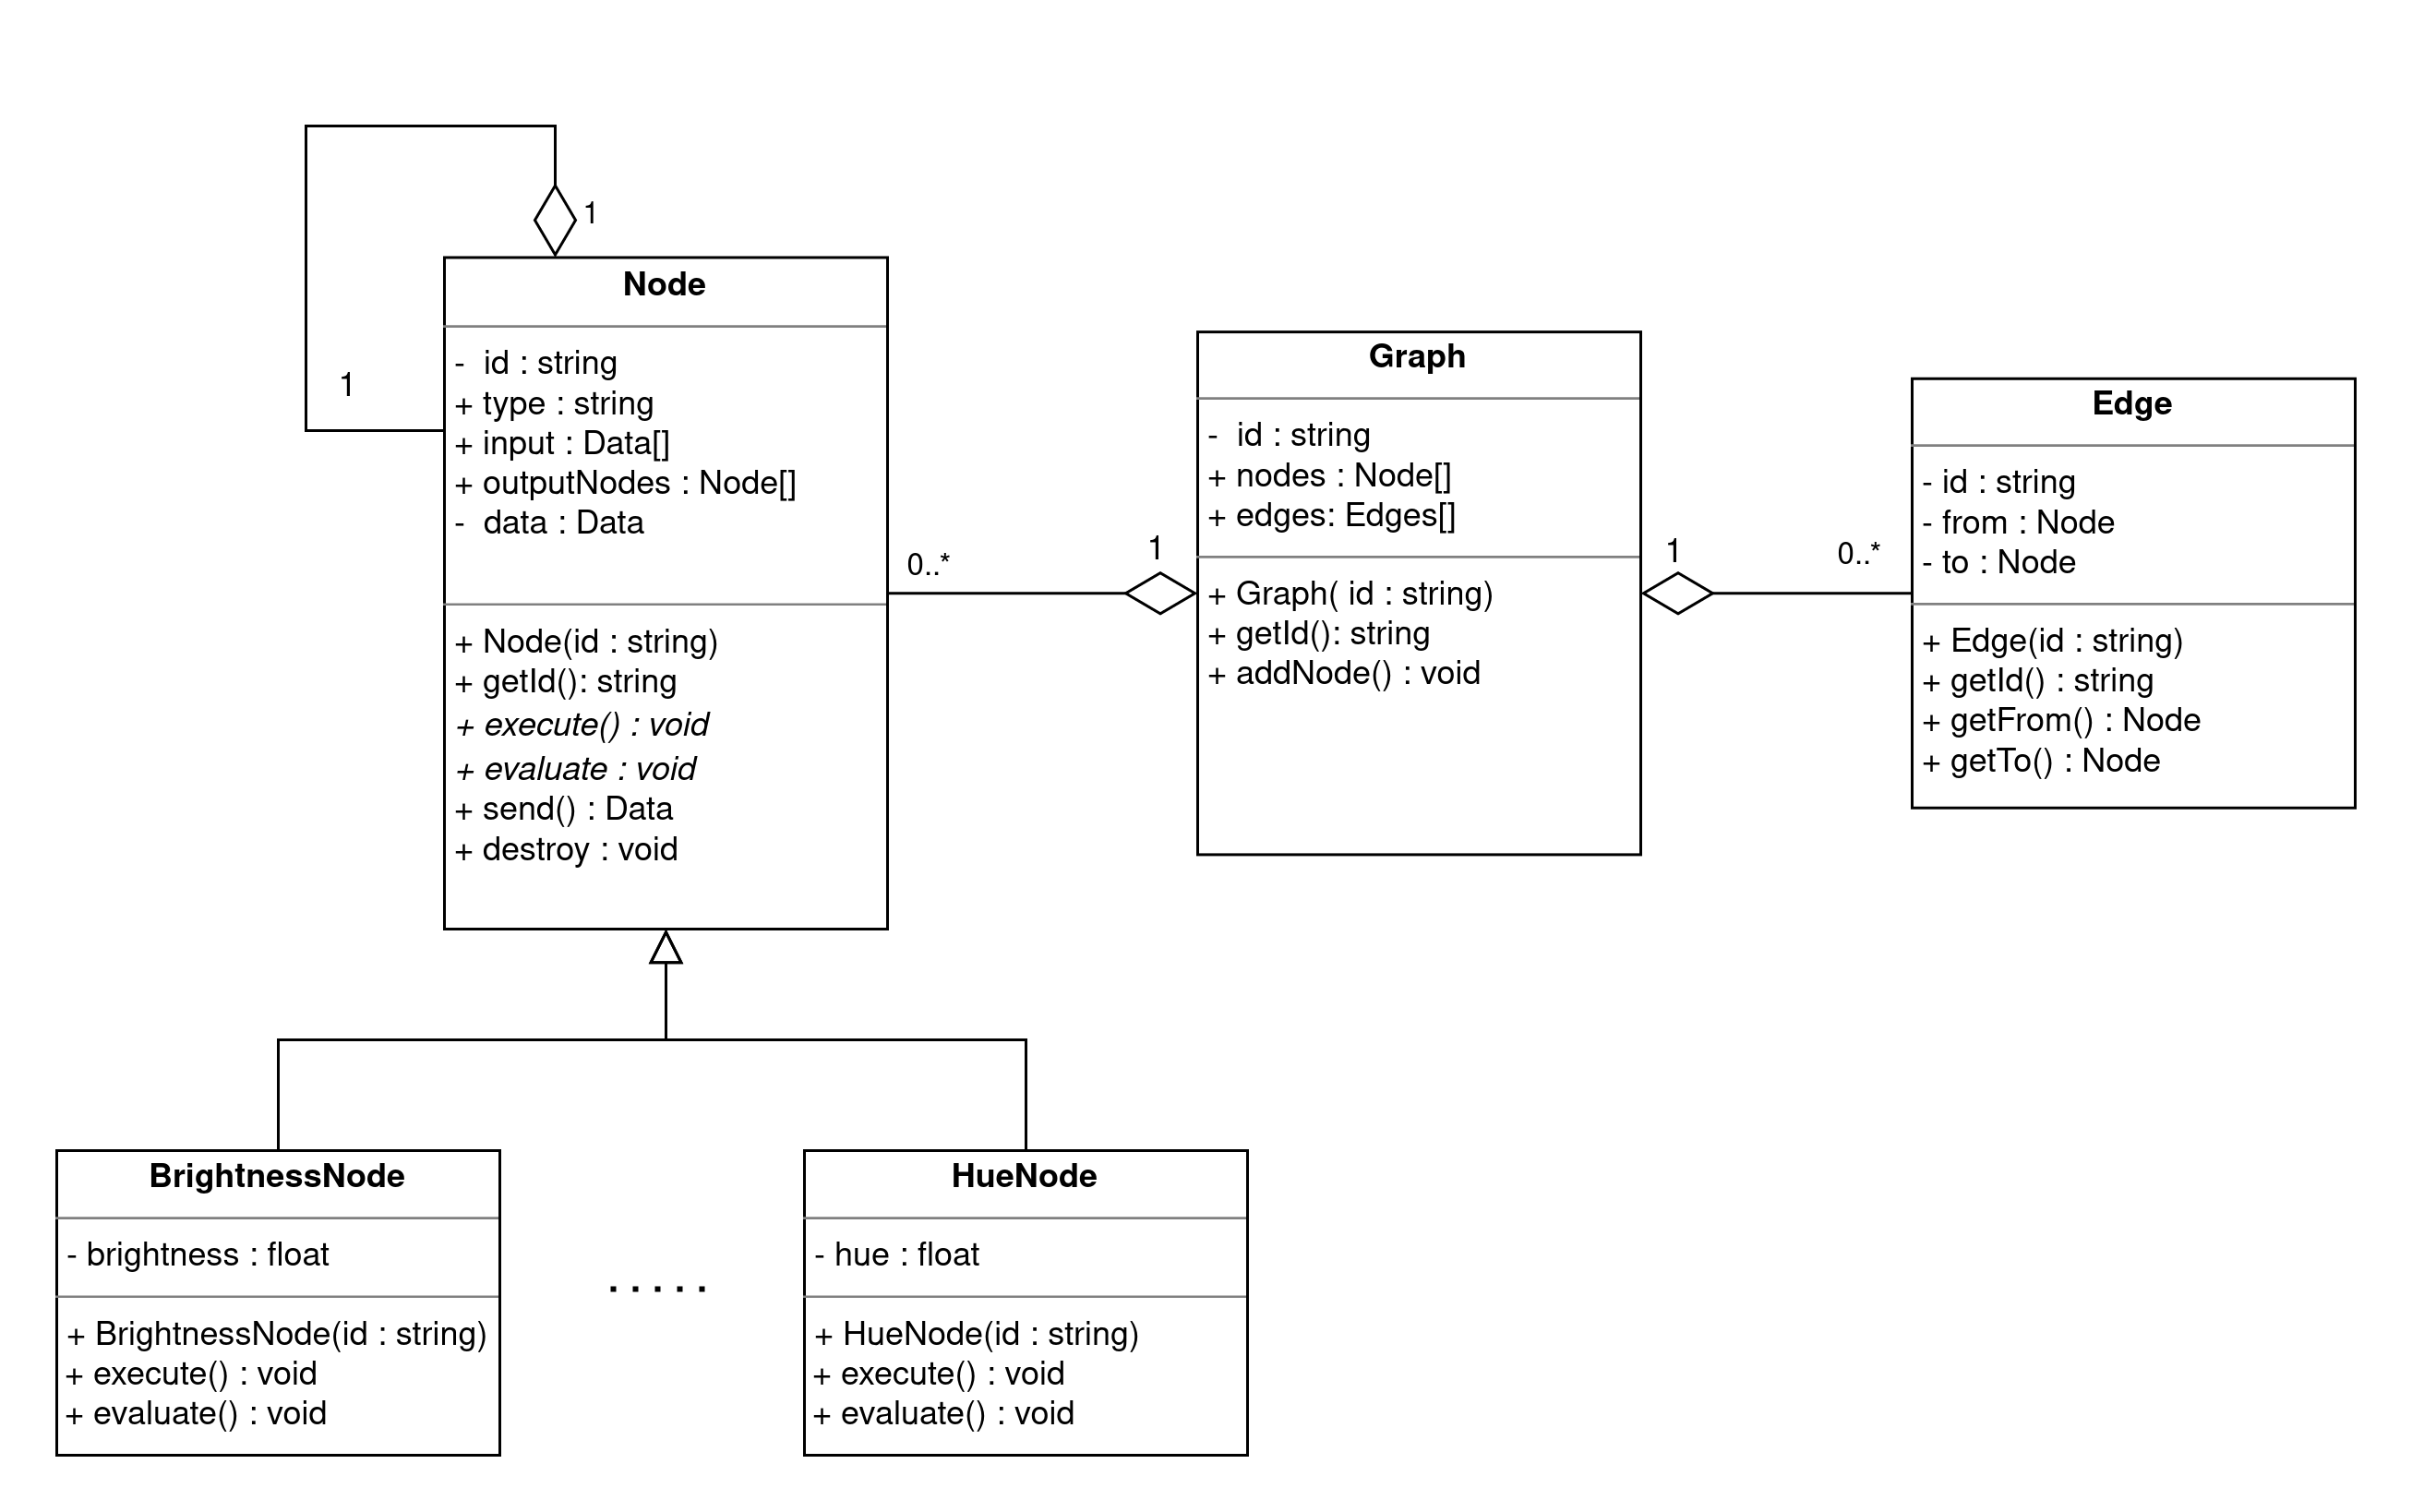
\includegraphics[width=0.8\textwidth]{../diagramPng/Graph-Subsystem.png}}
\end{figure}


\addcontentsline{toc}{subsection}{NLP Subsystem}
\subsubsection*{NLP Subsystem}
\begin{figure}[htbp]
    \centering
    \href{https://drive.google.com/drive/u/2/folders/1rnYMSGTOmKY8_pOyJUIacjTxuubO_6NX}
    {\includegraphics[width=0.61\textwidth]{../diagramPng/Graph Parsing-Subsystem.png}}
\end{figure}

\pagebreak
\addcontentsline{toc}{subsection}{User Management Subsystem}
\subsubsection*{User Management Subsystem}
\begin{figure}[htbp]
    \centering
    \href{https://drive.google.com/drive/u/2/folders/1rnYMSGTOmKY8_pOyJUIacjTxuubO_6NX}
    {\includegraphics[width=0.95\textwidth]{../diagramPng/User-Subsystem.png}}
\end{figure}

\pagebreak

\addcontentsline{toc}{section}{Functional Requirements}
\section*{Functional Requirements}

\addcontentsline{toc}{subsection}{Requirements}
%I split these up but idk, probs wrong sus
\subsection*{Requirements}

Requirements with a \textbf{*} next to it represents optional and \textit{nice
to have} requirements.

\begin{enumerate}[label=\arabic*.]
    \item Project Management
    \begin{enumerate}[label*=\arabic*.]
        \item Users should be able to import a single photo as well as multiple photos. 
        \item The system should be able to export the unedited images and the edited images.
        \item The system should store projects and retrieve projects from local storage.
        \item The system should be able to sync projects to the cloud. \textbf{*}
        \item The system should allow the user to revert changes.
        \item Users should be able to efficiently switch between and work on multiple projects.
        \item Users should be able to share their projects, images, and graphs.
    \end{enumerate}
    
    \item Layout
    \begin{enumerate}[label*=\arabic*.]
        \item Users should be able to view the changes they made to the original image,
        either with a button or slider.
        \item With the use of image segmentation the users should be able select
        objects in the image by pressing on the object.
        \item Users should be able to customize the layout tiles to fit their preference.
        \item System should be able to display multiple graphs and photos
        \item System should have a command palette to to provide easy access to tools.
    \end{enumerate}

    \item Graph Management
    \begin{enumerate}[label*=\arabic*.]
        \item Add nodes
        \item Remove nodes
        \item Manipulate node positions
        \item Anchor nodes to each other to create a logical data flow
        \item Change the properties and values of nodes
        \item System should contain a collision detection algorithm to
        place the nodes on the graph
        \item Cycle detection algorithm to indicate invalid connections
    \end{enumerate}
    
    \item Natural Language Processing to Graph \textbf{*}
    \begin{enumerate}[label*=\arabic*.]
        \item Generated graph should conform to a specific grammar
        \item User should be able to describe an edit the image.
        which should be processed to generate a functional graph.
    \end{enumerate}
    
    \item Photo Processing and Graph Interpreter
    \begin{enumerate}[label*=\arabic*.]
        \item The system should be able to support multiple different image formats/file
        types, such as jpeg, png, svg etc 
        \item Users should be able to edit the photos manually with the standard 
        features such as adjusting the white balance, hue, and exposure etc. 
        \item Users should be able to edit a selected object in the image the 
        same way one would edit the rest of the image. 
        \item System should be able to do object segmentation.
    \end{enumerate}

    \item User Administration
    \begin{enumerate}[label*=\arabic*.]
	\item Register and sign in with multiple providers
	\item View and manage account details
	\item View and manage list of projects
	\item Manage syncing of projects, layouts and user settings across multiple
	devices\textbf{*}
    \end{enumerate}
\end{enumerate}

\addcontentsline{toc}{subsection}{Subsystems}
\subsection*{Subsystems}
\begin{enumerate}
    \item Project Management
    \item Layout
    \item Graph Management
    \item Natural Language Processing to Graph
    \item Photo Processing \& Graph Interpreter
    \item User Administration
\end{enumerate}

\pagebreak

\addcontentsline{toc}{subsection}{Use Case Diagrams}
\subsection*{Use Case Diagrams}

\subsubsection*{Project Management Subsystem}
\begin{figure}[htbp]
    \centering
    \href{https://drive.google.com/drive/u/2/folders/18FJi5U-PEzTiB-SsYfPQOV304R0K7s3H}
    {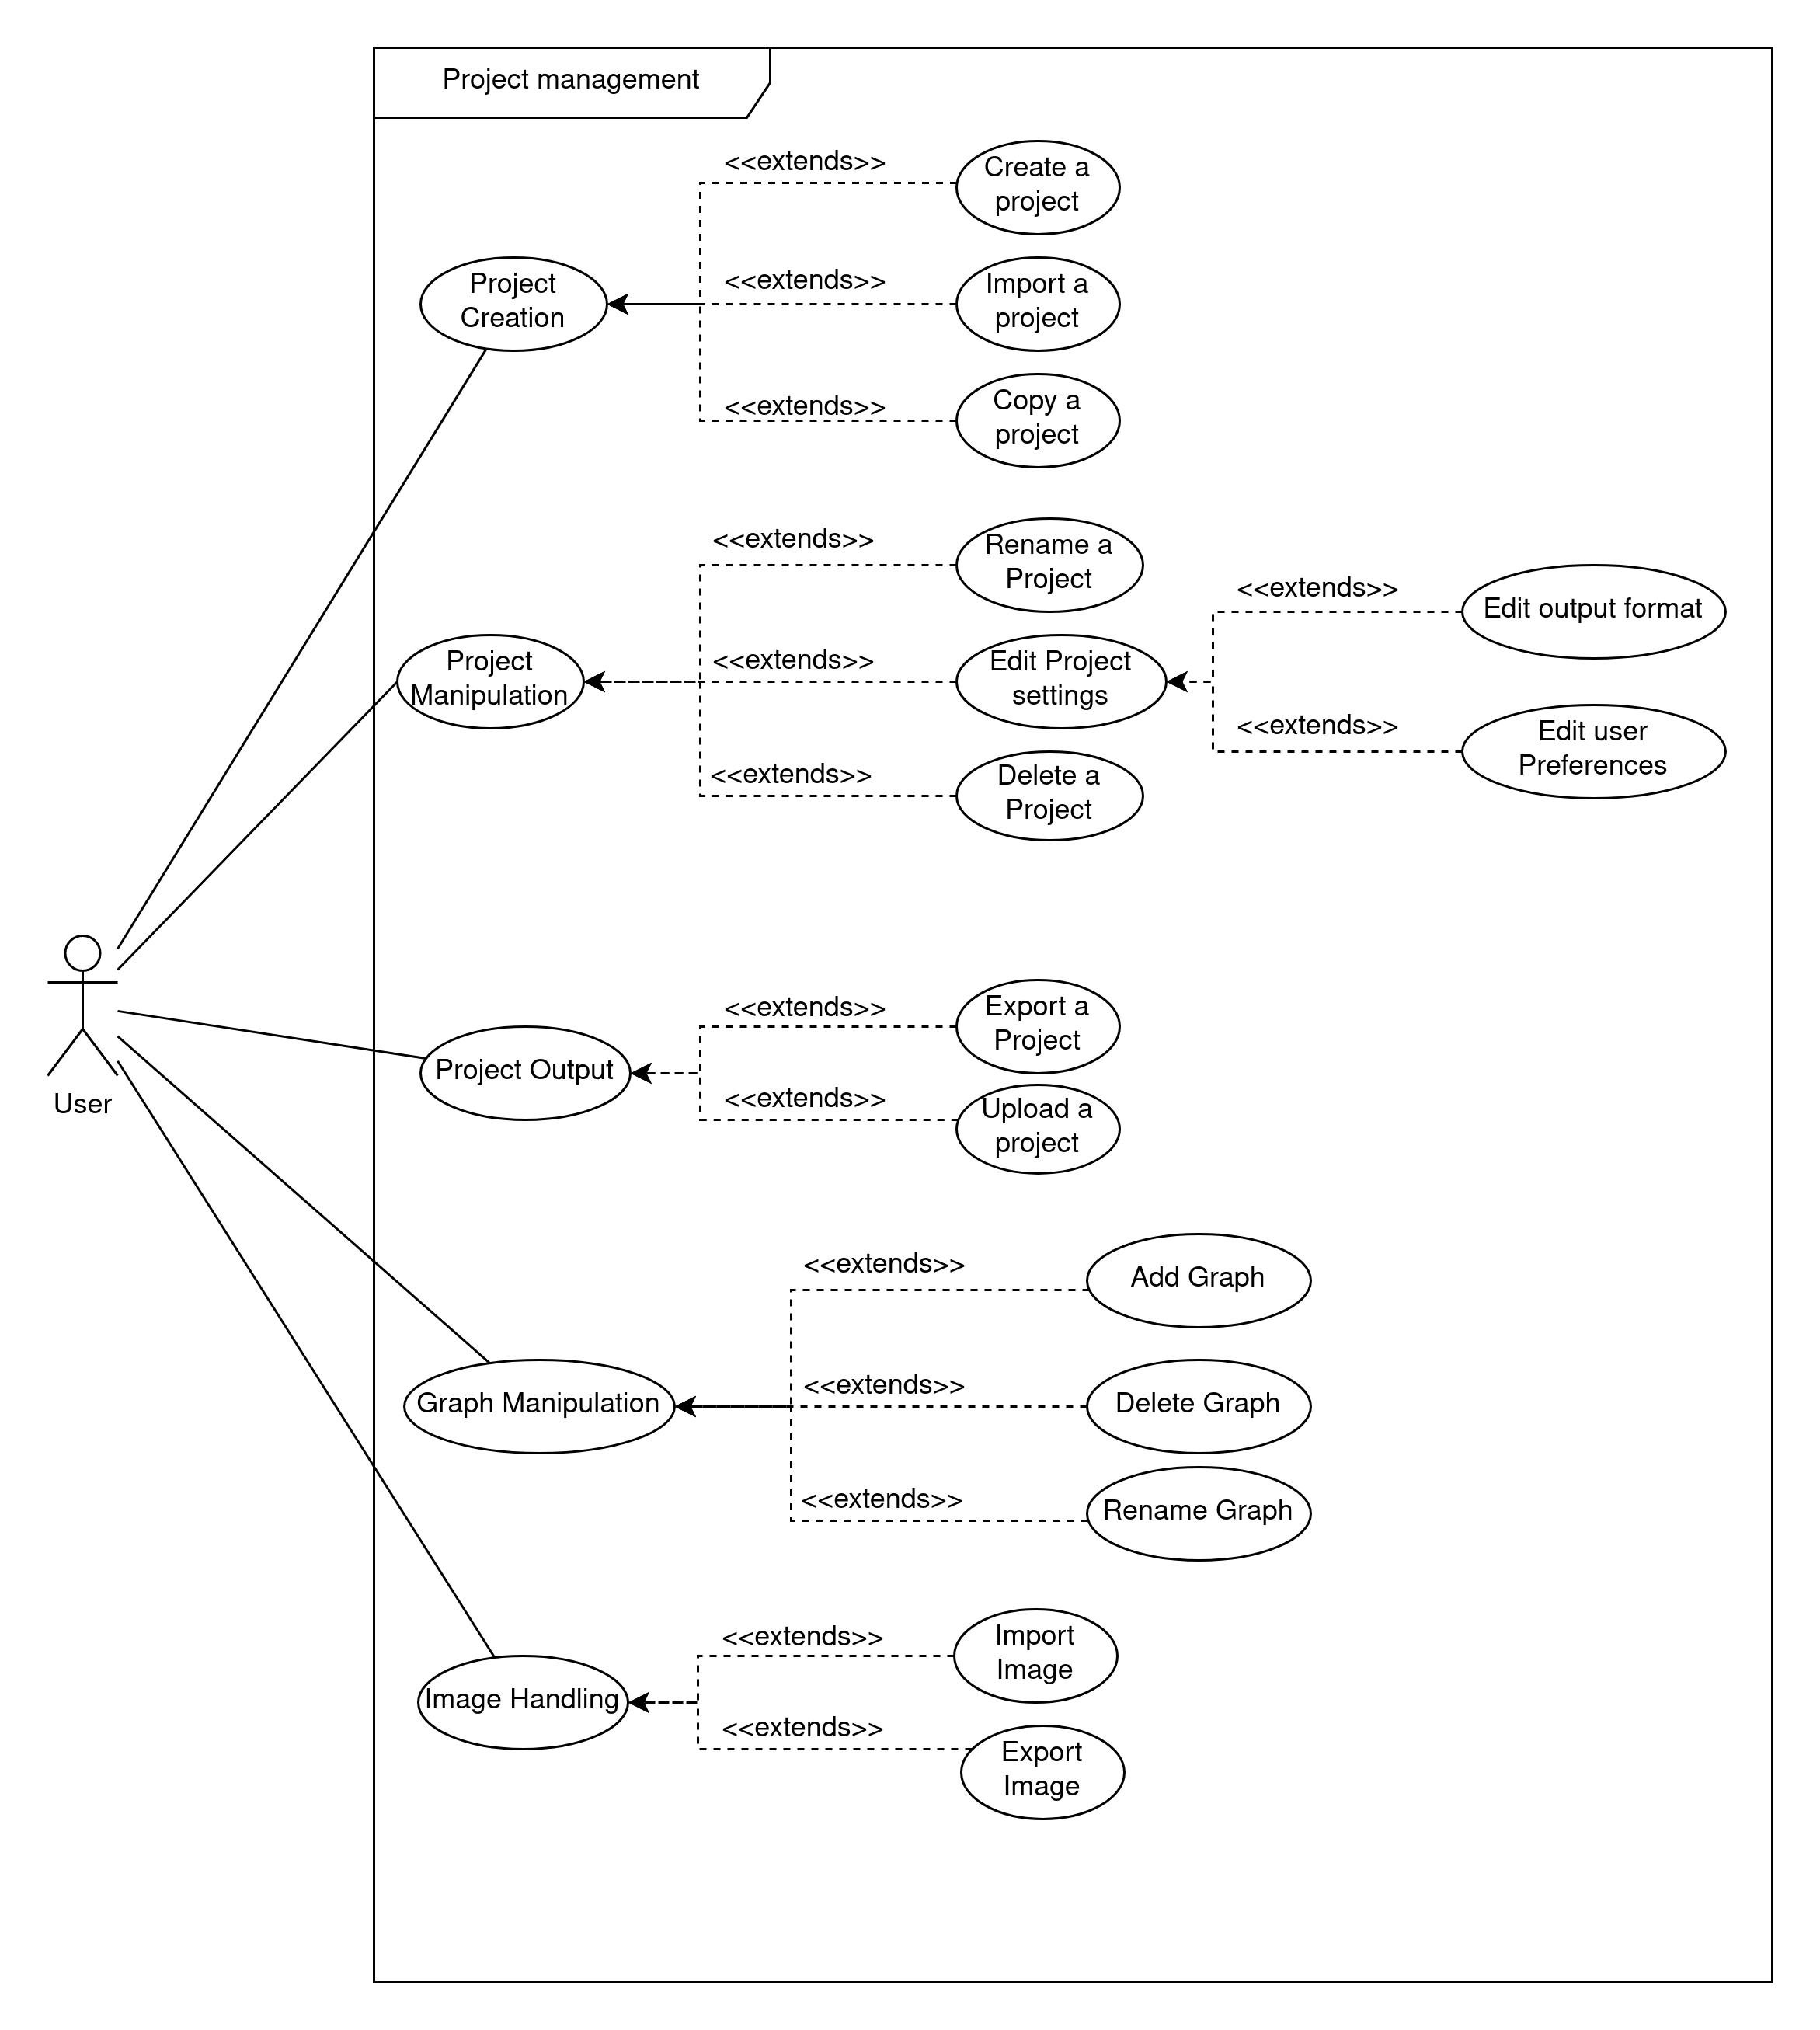
\includegraphics[width=1\textwidth]{../diagramPng/Usecase Project-Subsystem.png}}
\end{figure}

\pagebreak
\subsubsection*{Layout Subsystem}
\begin{figure}[htbp]
    \centering
     \href{https://drive.google.com/drive/u/2/folders/18FJi5U-PEzTiB-SsYfPQOV304R0K7s3H}
     {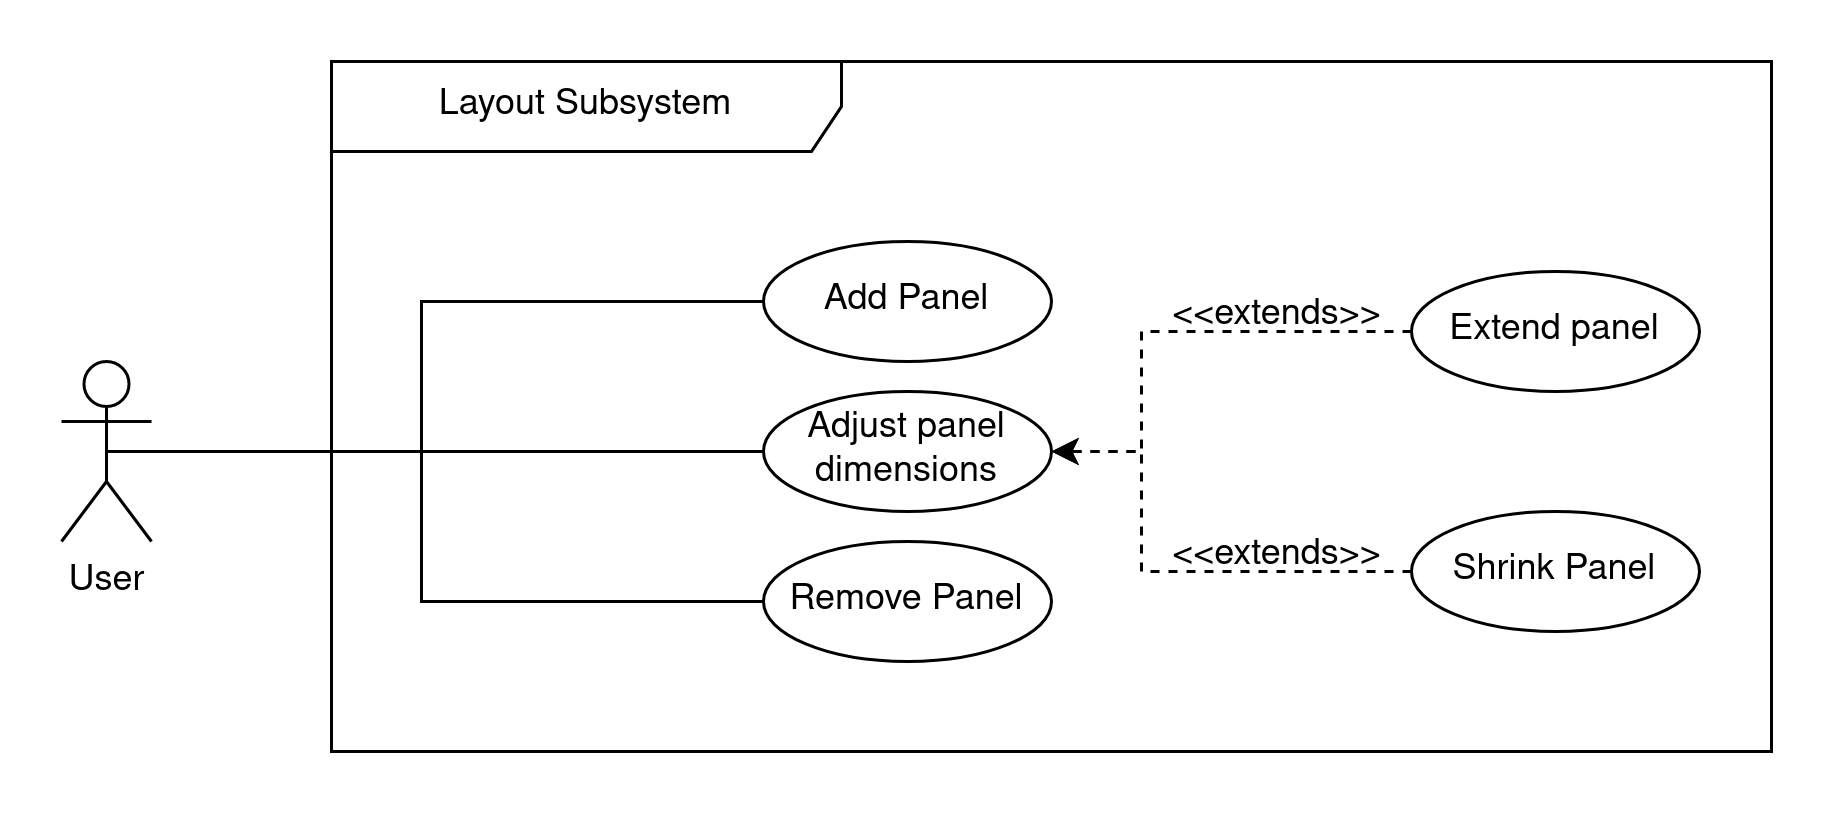
\includegraphics[width=1\textwidth]{../diagramPng/Usecase Layout-Subsystem.png}}
\end{figure}

\subsubsection*{Graph Management Subsystem}
\begin{figure}[htbp]
    \centering
    \href{https://drive.google.com/drive/u/2/folders/18FJi5U-PEzTiB-SsYfPQOV304R0K7s3H}
    {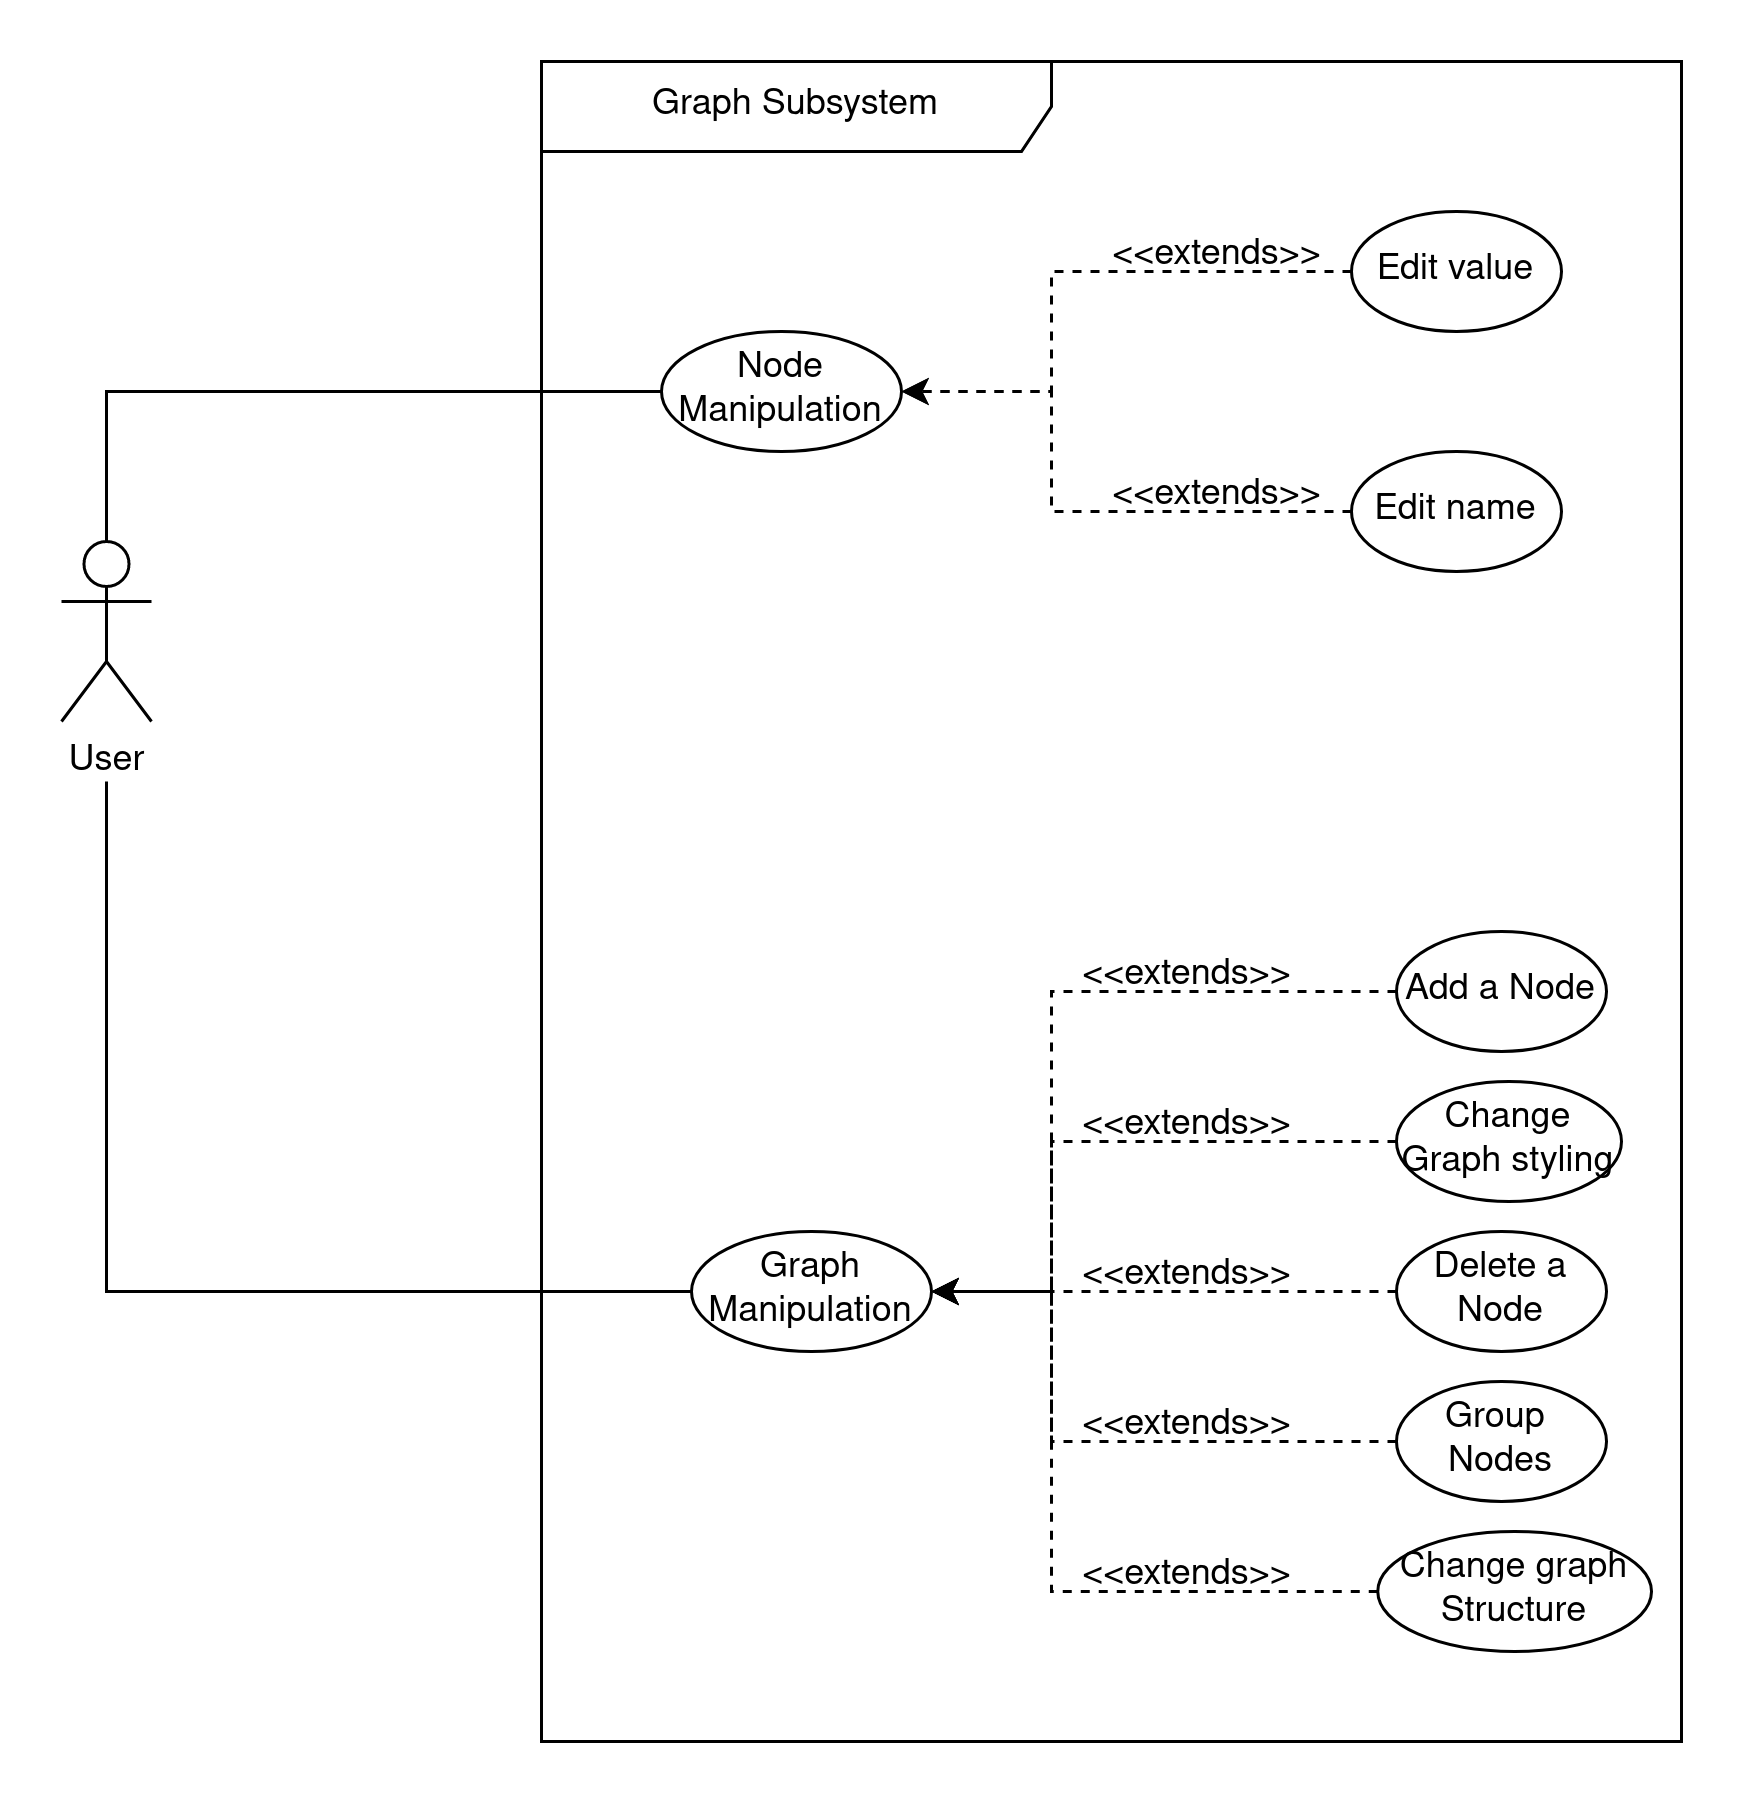
\includegraphics[width=0.6\textwidth]{../diagramPng/Usecase Graph-Subsystem.png}}
\end{figure}

\pagebreak
\subsubsection*{Image Processing Subsystem}
\begin{figure}[htbp]
    \centering
    \href{https://drive.google.com/drive/u/2/folders/18FJi5U-PEzTiB-SsYfPQOV304R0K7s3H}
    {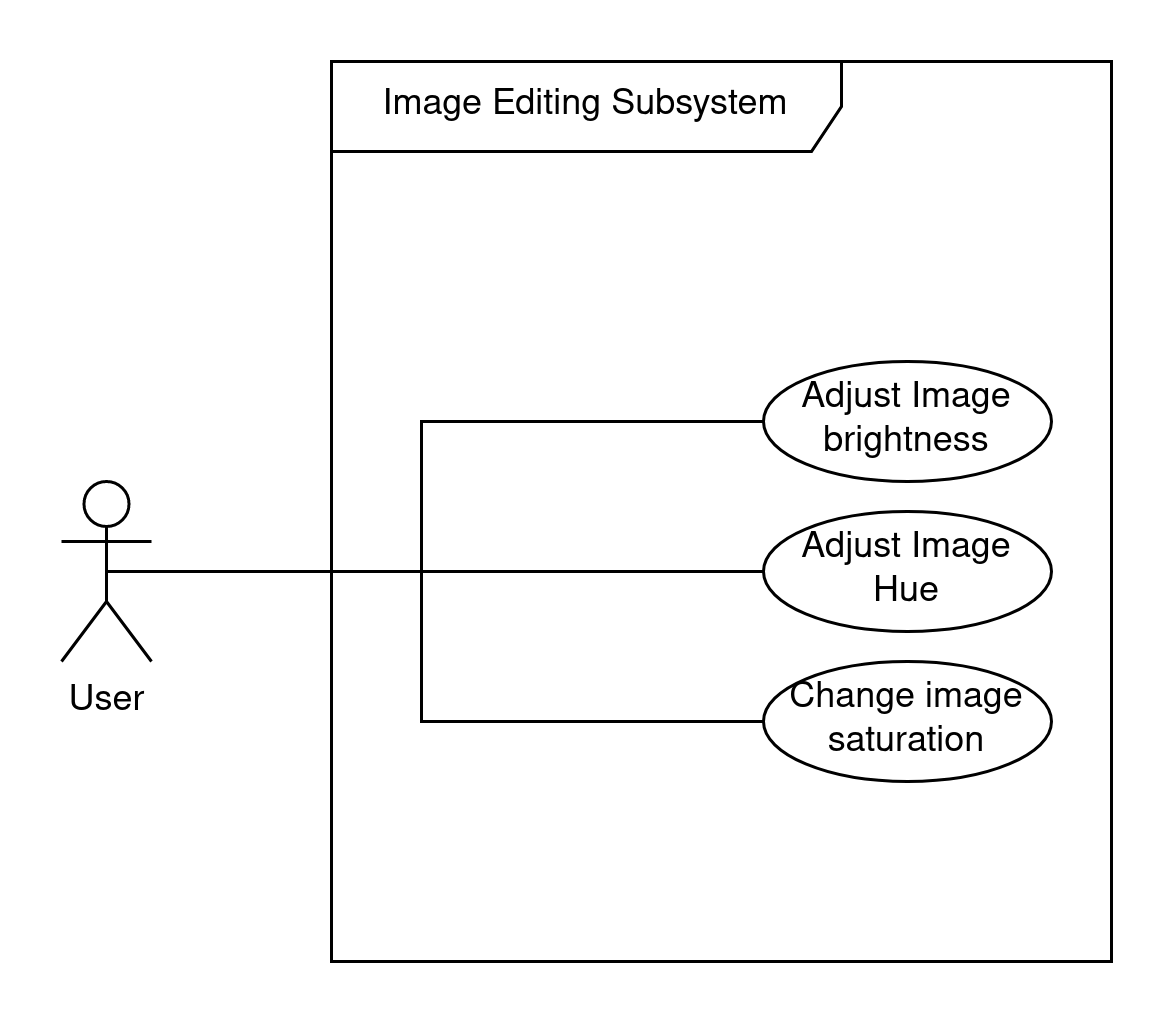
\includegraphics[width=0.6\textwidth]{../diagramPng/UseCase Image-Subsystem.png}}
\end{figure}

\subsubsection*{User Management Subsystem}
\begin{figure}[htbp]
    \centering
    \href{https://drive.google.com/drive/u/2/folders/18FJi5U-PEzTiB-SsYfPQOV304R0K7s3H}
    {\includegraphics[width=0.6\textwidth]{../diagramPng/Usecase User-Subsystem.png}}
\end{figure}


\pagebreak

\addcontentsline{toc}{section}{Quality Requirements}
\section*{Quality Requirements}

\subsection*{Performance}

The system should be able to handle large images and projects without
significant lag or delay.

The system should be able to process and apply image operations in real-time.

\subsection*{Reliability} 

The system should be able to recover from unexpected shutdowns or errors without
losing data.

The system should be able to store and retrieve images and projects reliably.

\subsection*{Usability} 
The system should be clear and concise on how it should be operated. 

The system must ensure that users can easily navigate and use the system without external assistance or unwarranted difficulty. All functionality must be properly documented such that high-end users can easily perform complex operations.

\subsection*{Security} 

The system must ensure that a user's information is kept safe and secure from malicious actors. Additionally the system itself must be properly protected such that the system can resist any and all attacks from 3rd parties and malicious users. 

\subsection*{Compatibility} 

The system should be compatible with all major operating systems such as
Windows, MacOS, and Linux.

The system should be compatible with all well-known image file formats.

\end{document}